\problemname{Pariserhjulet}
\begin{wrapfigure}{r}{0.3\textwidth}
	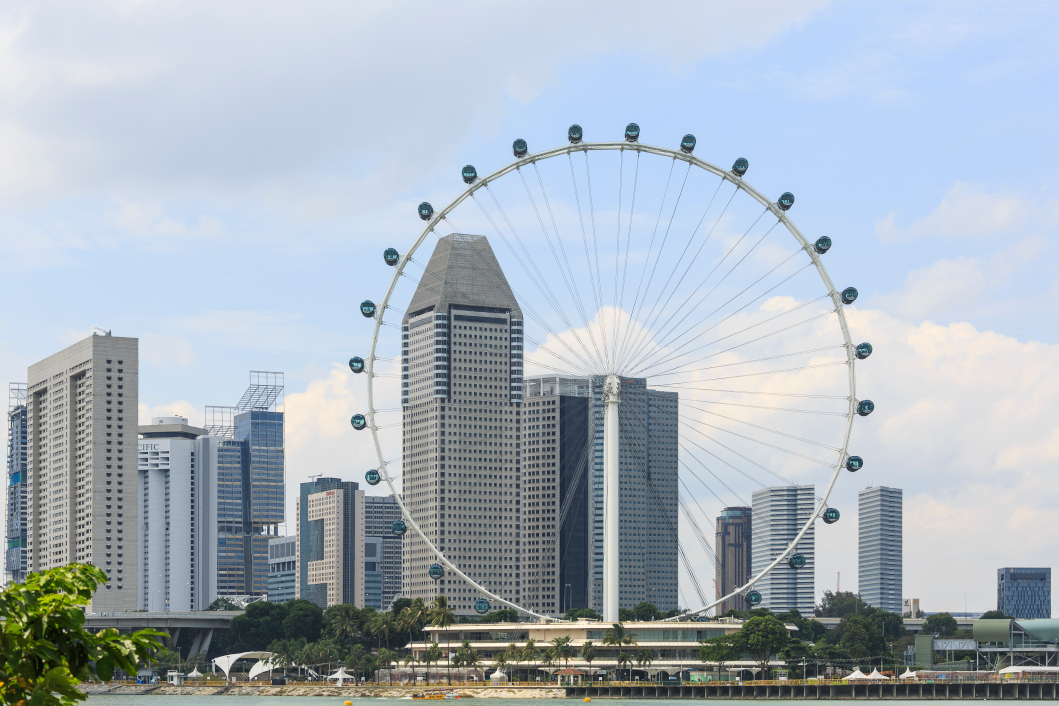
\includegraphics[width=0.3\textwidth]{image}
	\caption{\centering Singapore Flyer \newline © CEphoto, Uwe Aranas}
\end{wrapfigure}

Efter at have fulgt en meget veloptimeret rute gennem flyvepladsen er dit hold endelig ankommet til IOI i Singapore.
Under den første udflugt får alle $N$ hold på IOI lov til at køre i det gigantiske pariserhjul Singapore Flyer.
Pariserhjulet har $M$ vogne og skal bruge $M$ minutter for at dreje én omgang (med andre ord tager det 1~minut at flytte en vogn et skridt.)

Nogle hold er meget mere interesserede i at køre pariserhjul end andre, og derfor har hvert hold bestemt i forvejen, hvor mange runder de vil køre.
Idet af- og påstigning tager lang tid, er man også blevet enige om, at når et hold vel har sag sig i vognen, så bliver de siddende, indtil de har kørt alle deres runder.
Det betyder, at når hjulet drejer en vogn ned til indgangen, og vognen indeholder et hold, som vil fortsætte med at køre, så kan det næste holde ikke stige på.
Det næste hold bliver nødt til at vente på en tom vogn eller på et hold, som har kørt alle sine omgange og vil stige af.


Alle hold står lige nu i kø foran pariserhjulet, og det svenske hold vil vide, hvor lang tid der går, inden alle har kørt.

\section*{Indlæsning}
Første linje indeholder heltallene $N$ og $M$, adskilte af mellemrum, antallet af hold og antallet af vogne i pariserhjulet.
Anden række indeholder $N$ heltal $T_1$, $\ldots$, $T_N$, adskilte af mellemrum, hvor $T_i$ er antallet af omgange, som hold  nummer~$i$ vil køre.
Holdende står i køorden, og $T_1$ er første hold i køen.

\section*{Udskrift}
Udskriv en linje med et enkelt heltal, antallet af minutter, det tager for at alle hold har kørt.

\section*{Begrænsninger}
Din løsning vil blive kørt på en række testgrupper, hver gruppe giver et vist antal point.
Hver testgruppe indholder flere testfald.
For at få point for en testgruppe skal du klare samtlige testfald i gruppen.
Dit endelige pointtal for problemet er det maksimale point for nogen af dine indsendelser.

\noindent
\begin{tabular}{| l | l | l |}
\hline
Gruppe & Point & Begrænsninger \\ \hline
1     & 20    & $1 \le N, M, T_i \le 100$ \\ \hline
2     & 30    & $1 \le N, M, T_i \le 1000$ \\ \hline
3     & 25    & $1 \le N, M \le 1000, 1 \le T_i \le 10^9$ \\ \hline
4     & 25    & $1 \le N, M \le 200,000, 1 \le T_i \le 10^9$ \\ \hline
\end{tabular}

\section*{Forklaring af eksempel 1}

\begin{figure}[h]
	\centering
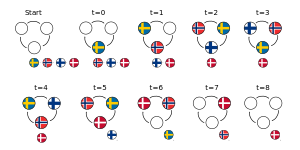
\includegraphics[width=0.8\textwidth]{sample1}
\caption{Eksempel 1}
\end{figure}

I eksempel~1 er der fire hold og tre vogne.
De fire hold, som på billedet er vist som Sverige, Norge, Finland og Danmark, vil køre henholdsvis 2, 2, 1 og 1 omgang.
Læg mærke til, at det danske hold ikke kan stige på pariserhjulet ved tid $t=3$ eller $t=4$, fordi hhv. det svenske eller norske hold allerede sidder i nederste vogn og vil køre en omgang mere.
